\section{Infrastructure}

\subsection*{Overview}
\frame{
\frametitle{What is a cluster?}
\framesubtitle{\includegraphics[height=0.3\textheight,width=\textwidth]{Titan1}}

\begin{columns}[T]
\column{.4\textwidth}
  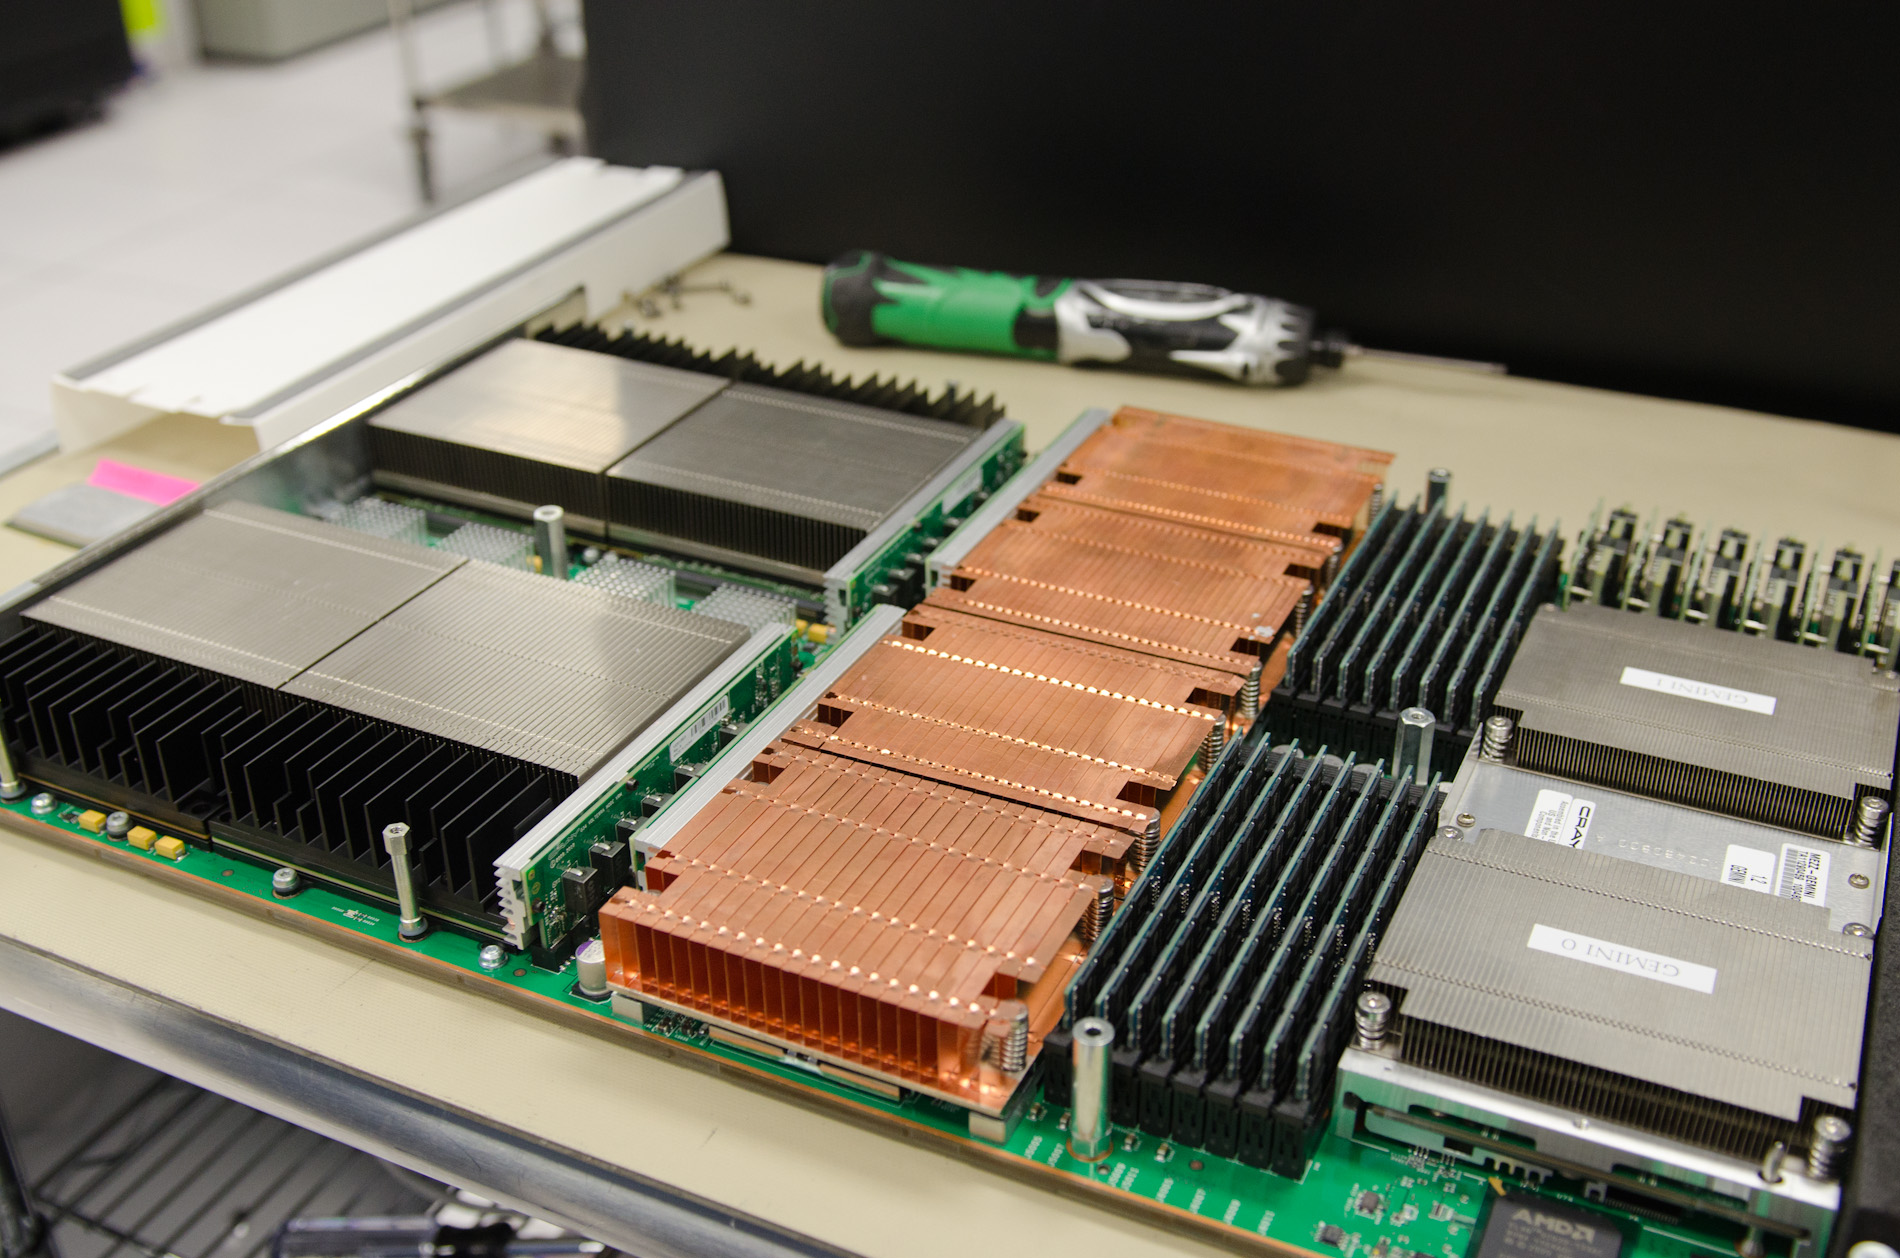
\includegraphics[width=\columnwidth]{TitanIn}
  \column{.3\textwidth}
  \begin{itemize}
    \item Cluster
    \item Racks
    \item Blades
    \item Nodes
    \item Processors 
    \item Cores
  \end{itemize}
\column{.3\textwidth}
  \begin{itemize}
    \item Login nodes
    \item Compute nodes
    \item Dedicated nodes
    \item Transfer nodes
    \item Service nodes
  \end{itemize}
\end{columns}
}


\subsection{Beskow}
\frame{
\frametitle{Beskow - Cray XC40 system}
\framesubtitle{\hspace{0.2\textwidth}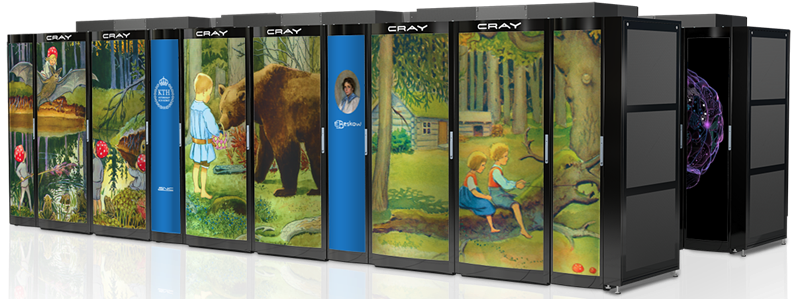
\includegraphics[height=0.3\textheight]{Beskow}}

\begin{alertblock}{}{\alert{Fastest machine in Scandinavia}}\end{alertblock}

\begin{columns}
\column{.6\textwidth}
  \begin{itemize}
    \item Lifetime: Q4 2018	
    \item $9$ racks $1676$ nodes
    \item Intel® Xeon® Processor E5-2698 v3\\ 40M Cache, 2.30 GHz
    \item $53.632$ cores - $32$ cores/node
    \item Aries Dragonfly network topology
    \item $104.7$ TB  memory - $64$ GB/node
   \end{itemize}
\column{.4\textwidth}
  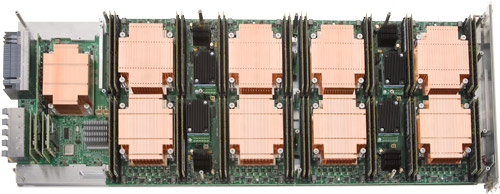
\includegraphics[width=\columnwidth]{xc30-blade}
  \scriptsize\\
  $1$ XC compute blade\\
  $1$ Aries Network Chip ($4$ NICs)\\
  $4$ Dual-socket Xeon nodes\\
  $4$ Memory DIMM / Xeon node
\end{columns}
}

\subsection{Tegner}
\frame{
\frametitle{Tegner}
\framesubtitle{pre/post processing for Beskow}

\begin{columns}
\column{.3\textwidth}
\scriptsize
  \begin{alertblock}{$5$ x $2$TB Fat nodes}
    $4$ x $12$ core Ivy Bridge\\
    $2$TB RAM \\
    $2$ x Nvidia Quadro K420
  \end{alertblock}
  
  \begin{alertblock}{$5$ x $1$TB Fat nodes}
    4x 12 core Ivy Bridge \\
    $1$TB RAM \\
    $2$ x Nvidia Quadro K420
  \end{alertblock}
  
  \begin{alertblock}{$55$ Thin Nodes}
    $2$ x $12$ core Haswell \\
    $512$GB RAM \\
    Nvidia Quadro K420 GPU
  \end{alertblock}
\column{.7\textwidth}
\normalsize
\centering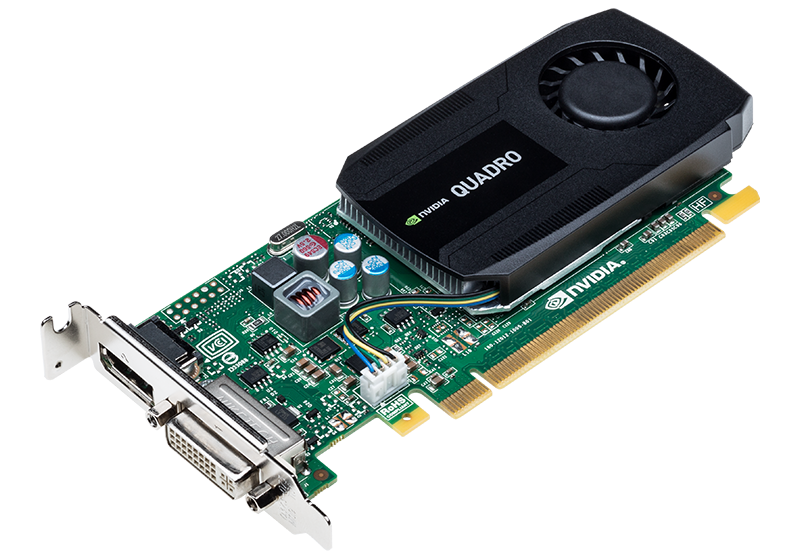
\includegraphics[width=.5\columnwidth]{k420}
  
  \begin{itemize}
    \item Used for pre/post processing data 
    \item Has large RAM nodes
    \item Has nodes with GPUs
    \item Lifetime: Q4 2018 
  \end{itemize}
\end{columns}
}


\subsection*{Summary}
\frame{
\frametitle{Summary of PDC resources}
\framesubtitle{}
\begin{table}
  \begin{tabular}{r|l|l}
   & \alert{Beskow} & \alert{Tegner}\\ \hline \hline
  Cores in each node &	$32$ & $48/24$\\\hline
  Nodes &	$1.676$ & 50 x  $24$ Haswell/GPU\\
  &&$10$ x $48$ Ivy bridge\\\hline
  RAM (GB) & $1.676$ x $64$	& $50$ x $512$GB\\
  && $5$ x $1024$GB\\
  && $5$ x $2$TB\\\hline
  Allocations &&\\
  (core hours per month)&&\\
  Small &	$<5k$&	$<5k$\\
  Medium &	$<200k$&	$<80k$\\
  Large &	$\geq 200k$	 \\\hline
  Allocation via SNIC &	yes &	yes\\\hline
  AFS &	login node only &	yes\\
  Lustre &	yes	& yes\\
  \end{tabular}
\end{table}
}

\subsection*{File systems}
\frame{
\frametitle{File Systems}
\begin{block}{Andrew File System (\alert{AFS})}
\begin{itemize}
  \item Distributed file system accessible to any running AFS client
  \item Home directory \\  \url{/afs/pdc.kth.se/home/[initial]/[username]}
  \item Access via Kerberos tickets and AFS tokens
  \item \alert{Not accessible to compute nodes on Beskow}
\end{itemize}
\end{block}

\begin{block}{Lustre File System (\alert{Klemming})}
\begin{itemize}
 \item Open-source massively parallel distributed file system
 \item Very high performance ($5$PB storage - $140$GB/s bandwidth)
 \item NO backup (always move data when done) NO personal quota
 \item Home directory \\  \url{/cfs/klemming/nobackup/[initial]/[username]}
\end{itemize}
\end{block}
}

\frame<presentation:0>[noframenumbering]{
\frametitle{File System Access}
 \begin{tabular}{ccc}
   
  \cellcolor{kthLightGreen} \textbf{AFS} & 
  \cellcolor{kthLightBlue}{Beskow Compute Node} &
  \cellcolor{kthLightBlue}\textbf{CFS}\\
   
  \cellcolor{kthLightGreen} Andrew File System & 
  \cellcolor{kthLightGreen!50!kthLightBlue} Beskow Login Node &  
  \cellcolor{kthLightBlue} Lustre File System\\ 
  
  \cellcolor{kthLightGreen}~ &
  \cellcolor{kthLightGreen!50!kthLightBlue}~ &
  \cellcolor{kthLightBlue}~\\

  \cellcolor{kthLightGreen} & 
  \cellcolor{kthLightGreen!50!kthLightBlue} Tegner Compute Node &  
  \cellcolor{kthLightBlue} \scriptsize{\url {/cfs/klemming/ }\alert{\textbf{nobackup}}\url{/}} \\
  
  
  \cellcolor{kthLightGreen} \scriptsize{\url{/afs/pdc.kth.se/home/}} & 
  \cellcolor{kthLightGreen!50!kthLightBlue} Tegner Login Node &  
  \cellcolor{kthLightBlue} \scriptsize{\url{/[initial]/[username]}} \\

  \cellcolor{kthLightGreen} \scriptsize{\url{/[initial]/[username]}}  &
  \cellcolor{kthLightGreen} &
  \cellcolor{kthLightBlue} \\

  \cellcolor{kthLightGreen} & 
  \cellcolor{kthLightGreen} KTH (Linux) computer &  
  \cellcolor{kthLightBlue} \scriptsize{\url{/cfs/klemming/}\alert{\textbf{scratch}}\url{/}}\\
 
  \cellcolor{kthLightGreen} &
  \cellcolor{kthLightGreen} & 
  \cellcolor{kthLightBlue} \scriptsize{\url{/[initial]/[username]}}\\
   
  \cellcolor{kthLightGreen} & 
  \cellcolor{kthLightGreen} Laptop/Home computer &
  \cellcolor{kthLightBlue}
  \end{tabular}
}

\frame<presentation:0>[noframenumbering]{
\frametitle{File System Access}
 
\begin{tikzpicture}
\begin{scope}[transparency group]
\begin{scope}[blend mode=multiply]
  \coordinate (AFS) at (1,0);
  \coordinate (CFS) at (4,0);
  \coordinate (LARGE) at (9,0);
  %\node at (3,-1) {\alert{\textbf{AFS}}}; 
  \node[align=center,text width=3.1cm] at (2.5,1.5) {\textbf{\alert{Tegner Login Node}}};
  \node[align=center,text width=3.1cm] at (2.5,0) {\textbf{Tegner Compute Node}};
  \node[align=center,opacity=1,text width=1.5cm] at (2.5,-2) {\textbf{Beskow Login Node}};
  
  \node[align=center,text width=2cm] at (6,0) {\textbf{Beskow Compute Node}};
  
  \node[align=left,text width=2.3cm] at (0,2) {\textbf{KTH (Linux) computer}};
  \node[align=center,text width=2.5cm] at (-1,-1) {\textbf{Laptop/Home computer}};
  
  \filldraw[fill=kthLightBlue, draw=black,opacity=0.5,rounded corners=1mm] (AFS) \irregularcircle{3.5cm}{3mm};
  \filldraw[fill=kthLightGreen, draw=black,opacity=0.5,rounded corners=1mm] (CFS) \irregularcircle{3.5cm}{2mm};
\end{scope}
\end{scope}
\end{tikzpicture}

  
}
